\documentclass[a4,12pt,oneside]{book}
%\usepackage{times}
\usepackage{algorithmic} 
\usepackage[algoruled]{algorithm2e} 
\usepackage{setspace}
\usepackage{url}
\usepackage{geometry}
\usepackage{graphicx}
\usepackage{subfigure}
\usepackage{epstopdf}
\epstopdfsetup{update}
\usepackage{makeidx}
\usepackage{float}
\geometry{tmargin=1 in,  bmargin=1 in, lmargin=1.5 in,  rmargin= 1 in}
\setcounter{secnumdepth}{3}
\setcounter{tocdepth}{3}
 \DeclareGraphicsRule{.eps}{pdf}{.pdf}{`epstopdf #1}

\makeindex

\pagestyle{plain}
%\textwidth 6in
%\textheight 9in

\begin{titlepage}
 \title{\bfseries\huge Scalable Flow Monitoring for Data Center}
  \author{A Dissertation Submitted in partial fulfillment of the degree of \\
    \\{\Large Master of Technology}\\in\\{\Large Computer Science}\\\\\\By\\\bf{Nirmoy Das}
  \vspace*{.2in}\\
    
\includegraphics[scale=0.5]{uoh.eps}\\ \\
	School of Computer and Information  Sciences\\
	University of Hyderabad, Gachibowli\\ 
	Hyderabad - 500046, India\\ \\
	Month, Year }
\end{titlepage}

\date{}

\renewenvironment{frontmatter}{\pagenumbering{roman}}{\newpage
  \pagenumbering{arabic}}
\renewcommand{\bibname}{Bibliography}
\newtheorem{algo}{Algorithm}[chapter]

\newenvironment{dedication}{
  \thispagestyle{empty}
  \clearpage\null\vfill
  \sl \hspace{1in}To,\\
  
  \hspace{1.5in}}{
  \vspace{3in}\vfill\null}


\def\prefacesection#1{%
  \chapter*{#1}
  \addcontentsline{toc}{chapter}{#1}
  \markboth{#1}{#1}}
\newenvironment{abstract}{\null\vfil\prefacesection{Abstract}}{\par\vfill\null}
\newenvironment{acknowledgments}{\null\vfil\prefacesection{Acknowledgments}}{\par\vfill\null}

\begin{document}
%\begin{large}
  \maketitle
 \onehalfspacing


\begin{frontmatter}
	{%certificate
	\thispagestyle{empty}
	\begin{center} 
		
\includegraphics[scale=0.5]{uoh.eps}
		\textbf{\Large CERTIFICATE}  
	\end{center}\vspace{.75in}

	{\sloppy This is to certify that the dissertation entitled ``\textbf{Scalable Flow Monitoring for Data center}'' 
    	submitted by \textbf{\mbox{Nirmoy Das}} bearing Reg. No. 11MCMT20, in partial fulfillment of the requirements for the award of Master of Technology in Computer Science, is a bona fide work carried out by him/her under my/our supervision and guidance.

	The dissertation has not been submitted previously in part or in full to this or any other University or Institution for the award of any degree or diploma. }\\ 

	\vspace{0.5in}
%	\parbox[t]{3in}
	{\flushright Anupama Potluri\\
	School of Computer and Information Sciences,\\
	University of Hyderabad\\}

	\vspace{1.0in}
%	\parbox[t]{3in}
	{\flushright Dean,\\
	School of Computer and Information Sciences,\\
	University of Hyderabad\\}
	}

\newpage
	{%declaration
	\thispagestyle{empty}
	\begin{center} 
		\textbf{\large DECLARATION}  
	\end{center}\vspace{.75in}

	{\sloppy I, \textbf{\mbox{Nirmoy Das}} hereby declare that this dissertation entitled ``\textbf{Scalable Flow Monitoring for Data center}
	'' submitted by me under the guidance and supervision of Dr. Anupama Potluri is a bona fide work. 
	I also declare that it has not been submitted previously in part or in full to this or any other University or Institution for the award of any degree or diploma. }\\ \\ \\ \\ \\ \\

	{\flushleft Date:   } 
	{\flushright Nirmoy Das\\
	Reg. No.: 11MCMT20\\
	\vspace{0.5in}
	Signature of the Student\\
	}
	}

    	\begin{dedication}
    	\thispagestyle{empty}
      		My Parents and Supervisor.
    	\end{dedication}
    
    	%\begin{acknowledgments}
      	%\paragraph\
I take this opportunity with immense pleasure to convey my gratitude to my supervisor, {\bf Ms. Anupama Potluri} who acted as a challenging captain coordinating all of our batch with great patience and invaluable suggestions. They really helped me to complete this task well before the stipulated time. She has always encouraged, supported, corrected and guided me during the project. This project happened to be one of my best journeys through core concepts of Computer Networks. The constant guidance of our supervisor helped me to develop both individually and professionally.\\

I can not get a better opportunity than this to thank profusely my senior {\bf Y. Jaya Lakshmi} with whose hard work my project literally became a cake walk. I would like to thank {\bf Tholoana Masupha} who is also part of this project. I am extreamly thankful to my lab mates {\bf B. Saritha, \bf B.Vishala and  \bf L. Ramprasad } for continuously inputting me with their valuable suggestions and being a source of encouragement at all possible times.  I would also like to thank the developers of {\bf ns2} for providing such a wonderful and robust software to work along with detailed documentation.\\

I am extremely grateful to our Head of Department, {\bf Prof. Arun Agarwal}, for providing excellent computing facilities and such a nice atmosphere for doing my project. I convey my heartfelt thanks to {\bf AI Lab staff} for their help in completing the project work successfully. \\

Last but not the least, I would like to express my heartful wishes to my beloved parents and my dear friends whose gracious solicitude helped me to complete this project successfully.  


\indent \indent \indent \indent \indent \indent \indent \indent \indent \indent \indent \indent \indent \indent \indent \indent \indent {\bf Sravanthi Bhavanam}
    	%\end{acknowledgments}
    
    	%\begin{abstract}
      	%\paragraph\
Mobile Adhoc Networks(MANETs) allow for infrastructure-less  mobile wireless networks to be established with minimal delay for deployment. The trend seen in applications of wireless services is that they make increasingly complex demands for Quality of Service(QoS). Thus, providing QoS in a MANET environment is becoming more important. However, QoS in MANETs is a challenging task, because of the inherent MANET limitations and properties. Some of the existing solutions are not scalable and have high signaling overhead. Some solutions are scalable but do not use the resources efficiently. Some solutions are simple but they do not even guarantee QoS and typically do not support multiple classes of service.
\paragraph\
Our proposed scheme is a cross-layer QoS-aware routing protocol that uses Diffserv model for data plane operations. It supports multiple classes of service and dynamically allocates resources for each QoS class. It reserves the resources for each flow and each flow is mapped to one of the QoS classes. The number of meters, policers and queues maintained per node are restricted to number of QoS levels only. So in this way it is scalable. As it reserves resources during route discovery process itself, it has less signaling overhead and has less latency to start data plane operations. To evaluate the performance of our scheme, we implemented it in the network simulator \textit{ns-2.29} by extending Dynamic Source Routing (DSR) protocol.
\paragraph\
Simulation results show that our scheme has achieved throughput close to ASAP while using fewer meters, policers and queues. Results also show that call acceptance ratio of our scheme is higher than ASAP. From the results we can also observe that our scheme gives QoS guarantee to the flows when congestion occurs whereas SWAN does not. Average end-to-end delay for our scheme is less than that of both ASAP and SWAN. Latency to start data plane operations is also acceptable in our scheme. Overall, we are performing better than ASAP and SWAN.
    	%\end{abstract}
    
    	\tableofcontents
    	\listoffigures
    	\listoftables
\end{frontmatter}
  
%\renewcommand{\baselinestretch}{1.7}
%\chapter{\label{chap:intro}Introduction}
%\paragraph\
 In computer networks the goal of QoS support is to achieve a more deterministic communication behavior, so that information carried by the network can be better preserved and network resources can be better utilized. QoS is an agreement or guarantee by the network to provide prespecified service attributes to the user in terms of delay, jitter(variance of delay), available bandwidth and probability of packet loss etc. QoS is essential to support real-time applications like VoIP, video conferencing, multimedia streaming etc. The Internet is, however, best-effort and does not provide any QoS. Many QoS models have emerged in recent times to support QoS in the Internet.

\section{QoS Models for Wired Networks}
\paragraph\
The two most popular QoS models for wired networks are
\begin{itemize}
\item Integrated services(Intserv).
\item Differentiated services(Diffserv).
\end{itemize}

\subsection{Integrated Services(Intserv)}
\paragraph\
The Integrated services model is the first standardized QoS model for the Internet. This model provides per flow QoS granularity. It reserves resources for each flow on the path by using Resource Reservation signaling protocol(RSVP) before commencing of the flow. The signaling messages carry QoS requirements of the flows. In this model per flow state information is maintained at the nodes and this information is refreshed periodically. At every node four basic components should be implemented. Those are signaling protocol, admission control, classifier and scheduler. It is well suited for meeting the dynamically changing needs of applications but it suffers from scalability problem.
 
\subsection{Differentiated Services(Diffserv)}
\paragraph\
 Diffserv is a fully distributed and stateless model. Instead of providing QoS at per flow granularity, Diffserv differentiates the traffic into a fixed number of classes. Diffserv aggregates a set of flows and applies a pre-defined behavior to that aggregate. So no state information for each flow is required to be maintained at any node. The network is divided into edge network and core network. The nodes at the edge of the network are responsible for classification of flows, policing them to ensure that the traffic complies with the agreement made by the service provider and marking the packets so that they can be differentiated in the core network. ToS field of the IP header is used for carrying marked codepoint. The nodes in the core network just check the codepoint of the packets and forward according to the per-hop behavior defined for that codepoint, making dataplane operations very efficient. 

\paragraph\
The raising popularity of multimedia applications among end users and the potential use of Mobile Adhoc Networks(MANETs) in civilian life have led to research interest in providing Quality of Service support in MANETs. We are also concentrated on this research area. In the following sections we discuss about MANETs and their features, what are the challenges for providing QoS in MANETs and the existing solutions and their drawbacks.

\section{Mobile Adhoc Networks(MANETs)}
\paragraph\
A Mobile Ad hoc Network (MANET) is a collection of wireless mobile nodes dynamically forming a temporary network without the use of any existing network infrastructure or centralized administration. It is a multihop wireless communication network in which each node can either act as a host or a router. MANETs represent future generation wireless networks, capable of being deployed quickly and economically at places lacking any infrastructure. These characteristics make MANETs more suitable for defense based applications, disaster relief operations and commertial applications.

\section{Challenges for Providing QoS in MANETs}
\paragraph\
Providing QoS in MANETs is challenging because of the following reasons:
\begin{itemize}
\item \textit{Dynamic network topology:} Nodes are mobile in the network. Link breaks occur due to mobility of nodes. The flows which are using these links are disturbed and latency is involved in finding a new route. It is also possible that a new route may not be found. Thus QoS can be violated for such flows.
\item \textit{Interference and Noise:} Because of the wireless medium there is more interference and noise. Due to this packet losses may be more. So we can not guarantee QoS.
\item \textit{Limited battery life:} Nodes are power constrained. So QoS solutions should not be too complex which consume more processing power of nodes.
\item  \textit{Bandwidth-constrained:} Bandwidth is very limited in wireless networks. The estimation of available bandwidth is very difficult because it not only depends on admitted flows in the channel, but also on the neighborhood nodes.
\end{itemize}

\section{QoS Models for MANETs}
\paragraph\
All the proposed models either use Intserv or Diffserv properties and these are mainly categorized as 
\begin{itemize}
\item Cross-layer solutions.
\item Independent solutions also known as frameworks.
\end{itemize}

\subsection{Cross-layer Solutions}
\paragraph\
QoS solutions can be provisioned at any layer in the protocol stack. Most existing schemes are at network layer. QoS-aware routing protocols will take QoS metrics as constraints to be satisfied, rather than trying to find the shortest path. Examples of these protocols are AQOR\cite{aqor}, ACOR\cite{acor}, QAODV\cite{qaodv} etc. A brief description of AQOR is presented in the next chapter.

\subsection{Independent Solutions}
\paragraph\
Instead of adding QoS to the routing or MAC layer, these schemes define separate QoS modules for signaling, admission control and scheduling etc. The main idea behind this is to separate functionality of each module so that these are independent to the routing or MAC protocols. Examples for these schemes are INSIGINA\cite{insignia}, ASAP\cite{asap} which are per flow QoS provisioning schemes and SWAN\cite{swan}, Diffserv framework\cite{diffframe} which are per class QoS provisioning schemes. We will discuss some of these frameworks in the next chapter.
 
\section{Motivation}
\paragraph\
From our literature survey, we find that the problems with existing QoS solutions for MANETs are
\begin{itemize}
\item Some are not scalable \cite{asap}, \cite{aqor}, \cite{insignia}.
\item A few have high signaling overhead \cite{asap}, \cite{ceqmm}.
\item There is no QoS guarantee\cite{swan}, \cite{asap}.
\item Many of the scalable schemes use static resource allocation which leads to waste of resources if there are no flows of tat QoS level\cite{diffframe}, \cite{ceqmm}, \cite{CLAD}.
\item Some of the schemes do not support multiple classes of services\cite{swan}, \cite{diffframe}.
\end{itemize}

\paragraph\
So, we proposed a cross-layer QoS aware routing protocol that supports multiple classes of service. It dynamically allocates resources for each QoS class. It reserves the resources for each flow and each flow is mapped to one of the QoS classes. The number of meters, policers and queues maintained per node are restricted to number of QoS levels only. So in this way it is scalable. As it reserves resources during route discovery process, it has less signaling overhead and the latency to start data plane operations is reduced. In addition, we use Diffserv principle of marking packets at the source(which is treated as an edge router) and simply enqueueing in the right queue at the intermediate routes speeding up processing in the data plane. To evaluate the performance of our scheme, we implemented the scheme in the network simulator \textit{ns-2.29} by extending Dynamic Source Routing (DSR) protocol which is an on-demand routing protocol for MANETs. We also ported the freely available implementations ASAP and SWAN to \textit{ns-2.29} for comparison of the performance of our scheme with them.
\paragraph\
Our simulation results show that the objectives with which we proposed our solution like scalability, high call acceptance ratio and QoS guarantee etc. are achieved.


\section{Organization of the Project Report}
\paragraph\
The rest of the project report is organized as follows: In Chapter 2, we present some of the  existing QoS solutions for MANETs with their advantages and disadvantages. In chapter 3, we present our proposal and implementation details of our proposal in network simulator \textit{ns-2.29}. Actually we have extended Dynamic Source Routing Protocol(DSR) to be QoS-aware. So in this chapter we present what are the extensions required and how we achieved them. Simulation results of our scheme, ASAP\cite{asap} and SWAN\cite{swan} are given in chapter 4. Simulation results show that our scheme performs better than ASAP and SWAN. Finally we conclude with chapter 5.
\chapter{\label{chap:survey}Related Work}
\paragraph\
  Flow monitoring protocols like NetFlow\cite{NetFlow} and sFlow\cite{sFlow} can provide   important information about traffic that 
  passes through a network. However, contemporary  networking with its 10Gbps and higher NICs is outpacing the ability to monitor them 
  efficiently. As data centers are getting virtualized with virtual software switches and scaling to thousands  of nodes, 
  it is an immediate requirement to have monitoring systems that can scale effectively. There are not many solutions proposed that 
  provide scalable flow monitoring in data center networks. In this chapter, we review some of the literature that deals with scalable 
  flow monitoring in data center networks.
  
  \section{Edge Monitoring and Collection for Cloud (EMC2)\cite{emc2}} 
  \paragraph\
    Edge Monitoring and Collection for Cloud (EMC2) is a scalable network-wide monitoring service for data centers. 
    EMC2 stays inside the host computer  to monitor virtual switches. Monitoring at virtual switch is scalable due to 
    the distributed nature of the storage of the collected information.
    
  \subsection{Architecture}
    \begin{figure}[htb]
          \centering
          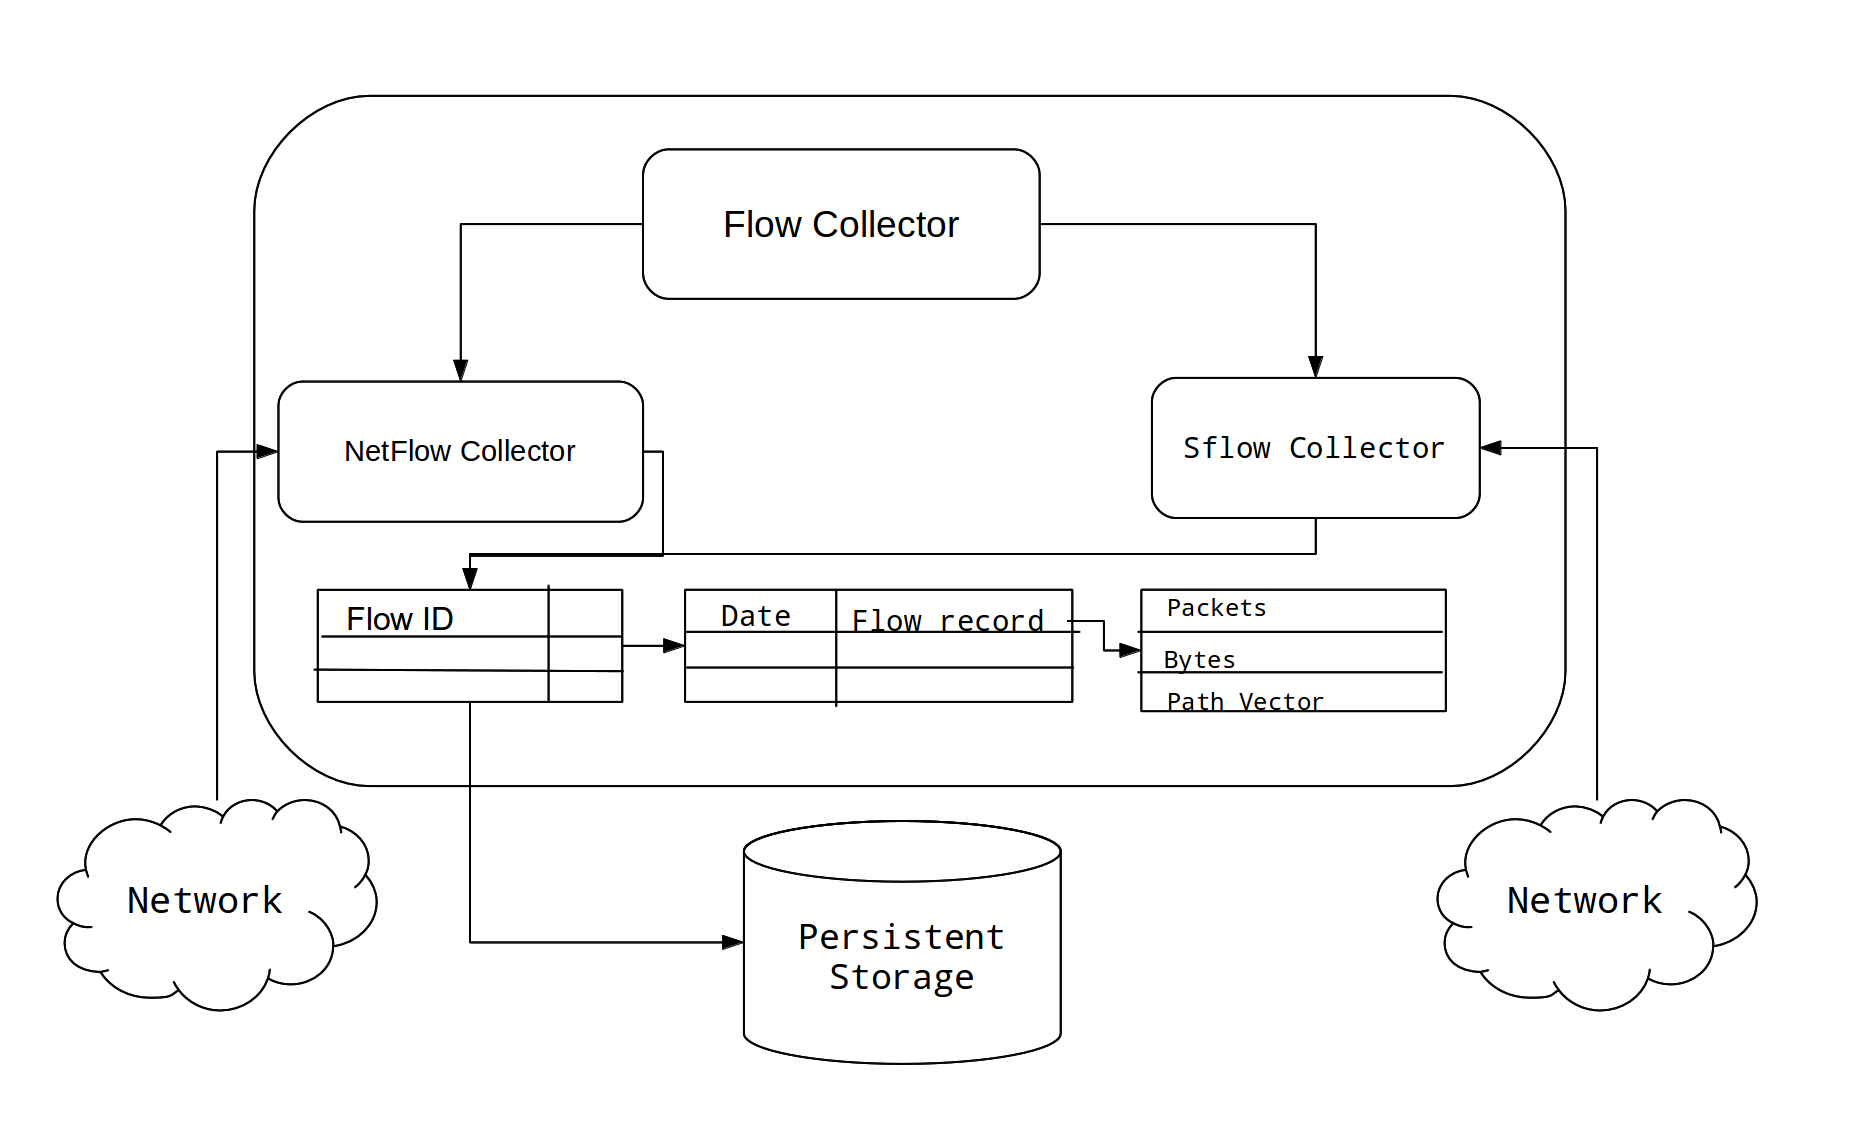
\includegraphics[scale=.35]{emc2.png}
          \caption{Architecture of EMC2.} 
    \end{figure}
    
    Figure 1.1 shows the architecture of EMC2.

    \paragraph\
    EMC2 is a multi-threaded application that contains the following modules:
    \begin{enumerate}
     \item Flow-Table : Flow-Table is an in-memory 2-level hash table.
     \item NetFlowParser : It parses the NetFlow datagrams and updates the Flow-Table.
     %AP: ``It'' is a singular pronoun. Should be associated with a singular verb ``parses'' not the plural verb ``parse''. Similarly ``updates'' and not ``update''. They update, it updates, she updaes, he updates and so on. Please use the proper singular noun/pronoun and verb combinations.
     \item sFlowParser : It parses the sFlow datagrams and updates the Flow-Table.
     %AP: Missing articles: you need to say ``the sFlow'' and ``the Flow-Table'' since you are talking about a specific entity. If you are talking in general, then you need to use the article ``a'' or ``an'' depending on whether the word starts with a consonant or a vowel resp.
     \item NetFlowCollector : It accepts the NetFlow datagrams and creates the parser thread upon receiving NetFlow datagrams.
     \item sFlowCollector : It does the same task like the NetFlowCollector but for sFlow datagrams.
     \item FlowCollector : It invokes two thread -- NetFlowCollector and sFlowCollector -- for accepting flow datagrams.
  \end{enumerate}


    \subsubsection{Flow-Table}
      \paragraph\
	Flow-Table is a 2-level in-memory hash table. The primary key for the hash table is the Flow ID which is formed based on the 
	layer 3 source and destination addresses. Flow ID maps to another hash table where timestamp is the key and flow record is the value. Each flow record contains number of packets, number of bytes and optional path vector.
%AP: Overuse of hyphen (-). Please do not hyphenate everything.

    \subsubsection{NetFlowParser/sFlowParser}
      \paragraph\
	NetFlowCollector and sFlowCollector create these two parser threads upon receiving a NetFlow/sFlow datagram respectively. 
	These parser threads parse the datagram and update the Flow-Table. They also perform two important tasks:
	%AP: ``Parser threads'' is plural - hence use the plural verb ``perform'' not the singular ``performs''. Also, do not keep on saying ``Parser threads''. You can say ``They'' after the first one or two sentences. It is obvious that ``they'' refers to the preceding reference whatever that may be.

	\begin{enumerate}
	 \item Deduplication.
	 \item Data rate prediction in presence of sampling.
	\end{enumerate}
   %AP: Use enumerate wherever possible as it gives you numbering. Bullets are used in more special cases such as primarily in slides etc.
   
   \paragraph{Deduplication:}
       Deduplication prevents duplicate flow records from being added to the Flow-Table. 
       %AP: Please see how I have modified the above sentence from what you had written.
       It uses the following algorithm.
       
       
     \begin{algorithm}[H]
        \caption{Detect Duplicate Flow}
	\label{alg1}

	\begin{algorithmic}
	  \IF{$flow-ID$ not exist}

	      \STATE add flow to the flow table.
	      \RETURN 

	  \ELSE 

	      \IF {Same exporter}
		  \STATE update the flow table.
		  \RETURN 

	      \ELSE

	        \STATE report duplicate flow.
	        \STATE update path vector.
	        \RETURN 

	      \ENDIF

	  \ENDIF

	\end{algorithmic}

       \end{algorithm}

    \paragraph{Data Rate Prediction in Presence of Sampling:}
       Sampling rate is specified in flow datagrams. Parser thread predicts the data rate by multiplying  sampling rate with the length 
       of the packet.
   %AP: This is not clear to me still and as I said does not convey what you told me. I will defer modification of this until I have read the paper.
   
    \subsubsection{NetFlowCollector/sFlowCollector}
      NetFlowCollector/sFlowCollector are collector thread that wait %(AP: wait not waits)
      for new NetFlow or sFlow datagrams and spawn a new NetFlowParser/sFlowParser thread upon receiving a datagram.
      
    \subsection{Advantages and Limitations}
    The authors state the following advantages of EMC2:

    \begin{itemize}
     \item Scalable monitoring as EMC2 monitors host $vswitches$ in a distributed fashion by storing the information as flat files in
     those hosts itself instead of sending them to a centralized collector.
     %AP: I hope the above is correct in terms of the content of the paper.
    \end{itemize}
    
    However, flat files are not really built for scalability unlike many other distributed databases available today such as Cassandra, 
    Big Table etc.. Therefore, it is not clear how much of performance can be obtained by storing the information in flat files in the host 
    itself. Considering that most data centers work with SANs rather than local disks, this may not be as scalable as claimed.
    
    %AP: There is a real problem with your references. But, I will look at how you wrote your .bib file etc. on Monday.

   \section{Scalable Internet Traffic Measurement and Analysis with Hadoop\cite{Lee}}
   \paragraph\
   Hadoop\cite{hadoop} is a distributed computing platform that uses distributed file system(HDFS) and MapReduce\cite{mapreduce} 
   programming model. Hadoop cluster consists of 
   commodity hardware that can scale  thousands of nodes to store huge amount of data. It can perform massive data analytics operations on 
   the available data using MapReduce. Storing NetFlow data on Hadoop and analysis using MapReduce offers scalable traffic 
   measurement and analysis.
   %Nirmoy:add images to describe Hadoop cluster and MapReduce 
    \subsection{Architecture}
     Traffic measurement and analysis system with Hadoop consists of following modules
     \begin{enumerate}
      \item Traffic collector.
      \item IP packet and NetFlow reader in Hadoop.
      \item Analysis in MapReduce.
      \item Interactive query interface with Hive\cite{hive}.
     \end{enumerate}

     \subsubsection{Traffic collector}
     \paragraph\
     Traffic collection is done by high-speed packet capture driver and load balancer. Load balancer forwards packets into
     multiple Hadoop DataNodes evenly. Traffic collector also can read trace files stored on the disk and writes them into HDFS. 
     Trace files contains Netflow packets or IP packets in $libpcap$ format.
     \subsubsection{IP packet and NetFlow reader in Hadoop}
     \paragraph\
      Storing binary trace file into Hadoop specific sequence file needs more computation power as every packet has to be sequentially 
      read from the trace file and stored into HDFS. Authors has developed new Hadoop APIs to store trace file directly into HDFS. 
      As there is no distinct mark to find out end of a packet records in $libpcap$ format, authors proposed a heuristic algorithm
      using timestamp-based bit pattern.

      \paragraph{Timestamp-based heuristic algorithm using MapReduce to identify packet records:}
	MapReduce job invokes multiple map tasks to process each HDFS block in parallel. Each of the map tasks follow these steps to
	identify packet records in HDFS block:
	\begin{enumerate}
	 \item Read two records using $libpcap$ 16-byte header.
	 \item Check timestamp value, that should be within duration of captured time.
	 \item Difference between wired packet length and captured length should be less then maximum packet length.
	 \item Check whether timestamp difference between two packet records within the define threshold. 
	\end{enumerate}
	
	\subsubsection{Analysis in MapReduce}
	Authors has implemented  MapReduce algorithms for processing IP packet as well as NetFlow packets.
	Here is the list of analysis tools
	\begin{enumerate}
	 \item IP Layer analysis provide following analysis jobs
	      \begin{enumerate}
	       \item Host and port count statistics.
	       \item Periodic flow statistics.
	       \item Periodic sample traffic statistics.
	      \end{enumerate}
	 \item TCP layer analysis compute following statistics
	       \begin{enumerate}
	        \item RTT.
	        \item Retransmission.
	        \item Throughput.
	       \end{enumerate}
	\item NetFlow analysis provides 
	      \begin{enumerate}
	       \item Human readable flow statistics.
	       \item Aggregated flow statistics.
	       \item Top N flows sorted by key such as packet count or byte count. 
	      \end{enumerate}

	\end{enumerate}

      \subsubsection{Interactive query interface with Hive}
      Hive is a data warehousing system build on the top of Hadoop that allows to generate MapReduce jobs using SQl like query.
      IP analysis MapReduce jobs process NetFlow packets on HDFS and  store flow record and IP statistics into
      Hive tables. A user can query on Hive tables using interactive web-based user interface.
      
      \subsection{Advantages and Limitations}
      Advantages of Hadoop based traffic  measurement and analysis are 
	\begin{enumerate}
	  \item Scalable storage.
	  \item MapReduce operations on flow data.
	\end{enumerate}
      Disadvantages of Hadoop based traffic  measurement and analysis are
	\begin{enumerate}
	 \item Low response time- ``the fasted MapReduce job takes 15+ seconds"\cite{mapreducetime}.
	 \item Hadoop NameNode was a single point of failure which solved in later version of 
	        Hadoop 2.0.0 with passive NameNodes.
	 \item Multiple NameNodes require to get high availability\cite{ha}.
	\end{enumerate}

	
      \section{\emph{nfdump\cite{nfdump}}}
      \paragraph\
      \emph{nfdump} provides set of tools to capture, analysis NetFlow packets. These set of tools are 
      \begin{enumerate}
	\item \emph{nfcapd}
	\item \emph{nfdump}
	\item NfSen 
       \end{enumerate}
      \emph{nfcapd} reads data from the network and stores them into disk. It also rotate the file to limit size of file.
      \emph{nfdump} allows $tcpdump$ style filter expression for processing NetFlow data stored by \emph{nfcapd} and display
      them on terminal or write into file. NfSen gives graphical overview of NetFlow data using RRDTool\cite{rrd};
        \begin{figure}[htb]
          \centering
          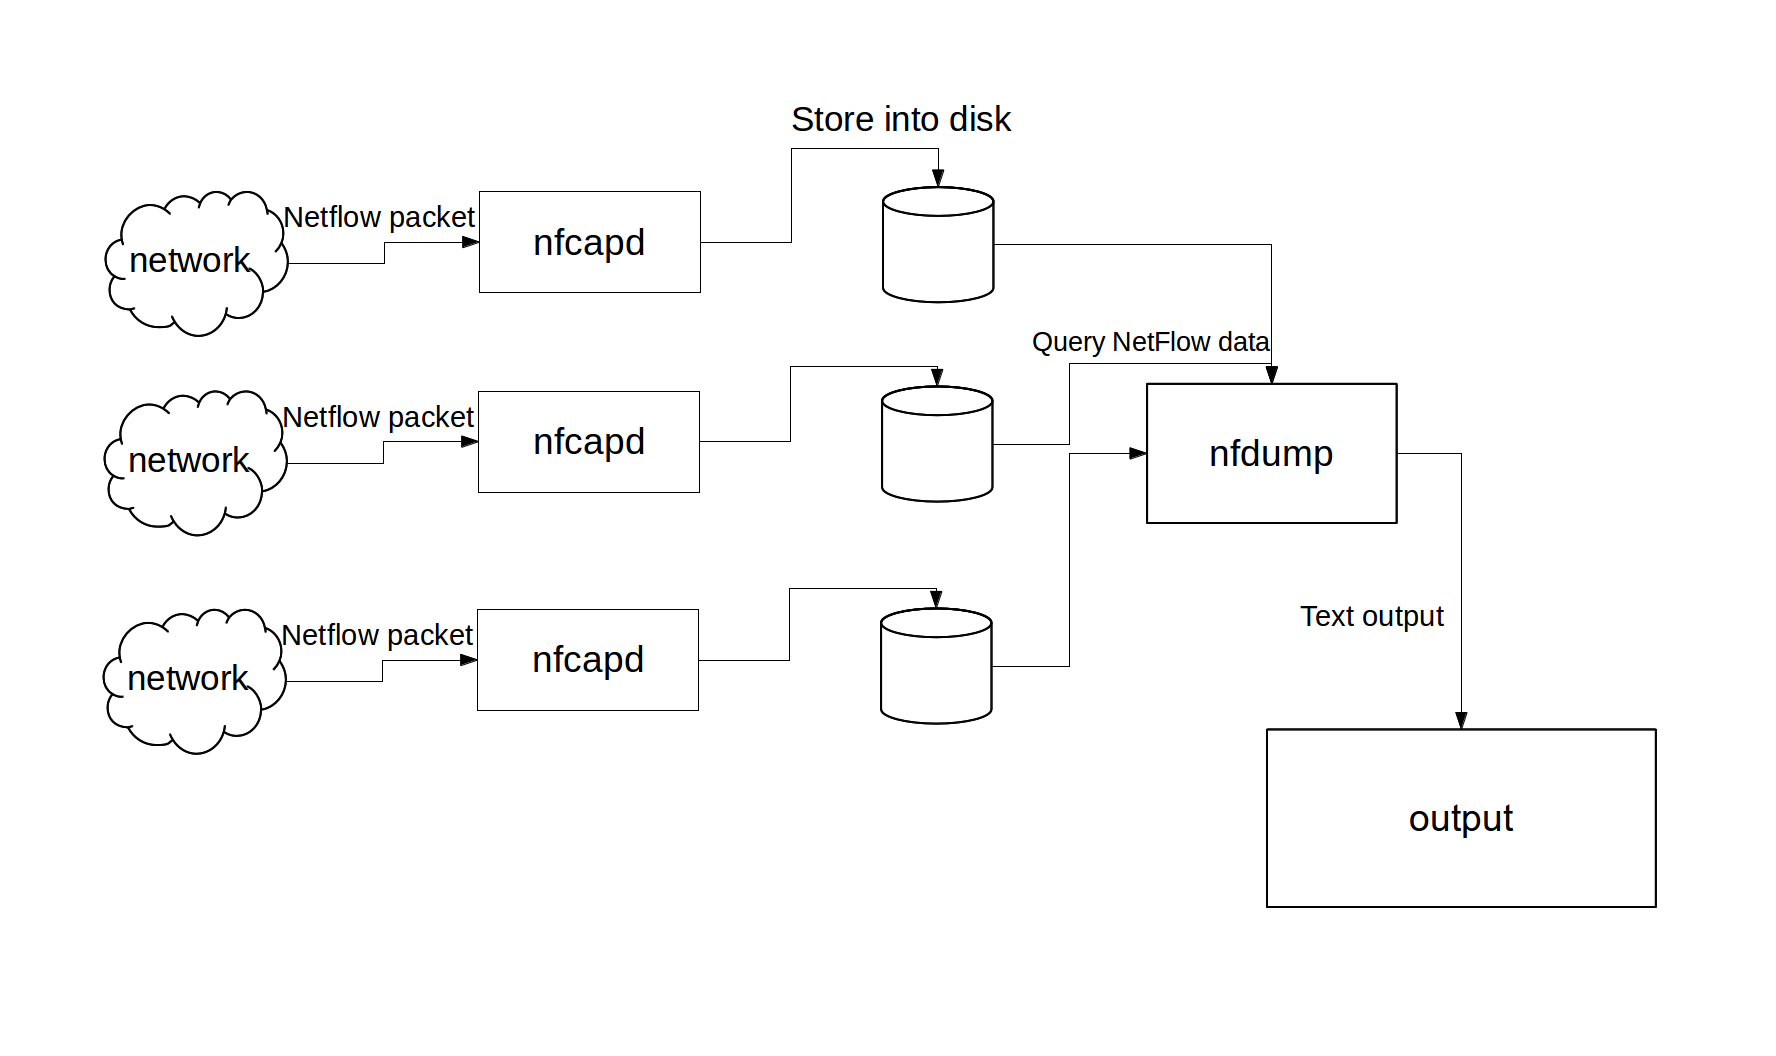
\includegraphics[scale=.35]{nfdump.png}
          \caption{Architecture of \emph{nfdump}.} 
	\end{figure}
      \subsection{Advantages and Limitations}
      \emph{nfdump} is suitable for small scale NetFlow analysis. In case of large scale NetFlow monitoring disk file 
      based storage is not sufficient.
      
      \section{Summary}
      In this section I have discussed  available solutions for scalable flow monitoring. The issues with current solutions are 
      \begin{enumerate}
       \item Lack of scalable storage.\cite{emc2}\cite{nfdump}.
       \item Lack of high availability data storage \cite{Lee}.
       \item Real-time flow analysis is difficult with current systems. \cite{Lee}  
      \end{enumerate}
      In the next chapter I describe design and implementation of modified \emph{ntop}(a NetFlow collector) that tries to solve
      few of the issues.

\chapter{\label{chap:our-idea} Cassandra plugin for \emph{ntop}}
\section{Overview}
  \paragraph\
    In this chapter I describe about \emph{ntop}, Cassandra and implementation of Cassandra plugin for \emph{ntop}.
    I also specify design and implementation of Cassandra client for C that developed using C-python API. I have done few 
    testing of my solution that I describe in results section. 
    
  \section{\emph{ntop}}
  \emph{ntop} is open-source traffic measurement application written in C. \emph{ntop} design follow UNIX philosophy:
  applications can be divided into small independent pieces that co-operate to achieve a common goal.
  \emph{ntop} has following module
    \begin{enumerate}
     \item Packet Sniffer - Capture packet using \emph{libpcap} library and also from UNIX sockets.
     \item Packet Analyzer - Analysis packet captured by Packet Sniffer.
     \item Traffic Rules - \emph{ntop} allows traffic rules for capturing packets to filter out unnecessary packets.
     \item Report Engine - Report Engine display analyzed output in an interactive web-based user interface. 
     \item Plugins - Using plugins anyone can extend \emph{ntop} to support extra features.
    \end{enumerate}
    
     \subsection{Packet Sniffer}
      \paragraph\
	Packet Sniffer captures packet using \emph{libpcap} library and store them into internal buffer, that helps to reduce packet drops
	in a busty traffic environment. \emph{libpcap} is supported by all major Operating Systems, that allows \emph{ntop} to be 
	portable to windows and UNIX variants.
        \begin{figure}[htb]
          \centering
          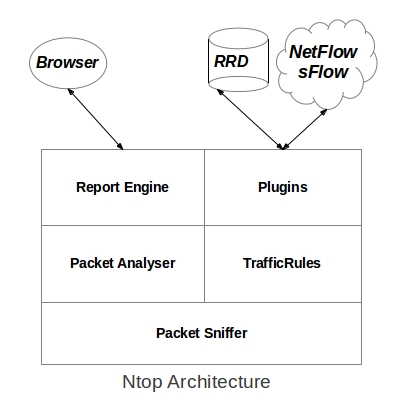
\includegraphics[scale=.5]{ntoparc.jpg}
          \caption{Architecture of \emph{ntop}.} 
        \end{figure}
	\subsection{Packet Analyzer}
	 \paragraph\
	 Packet Analyzer gets packets from Packet Sniffer and process those packets. Sniffed packets contained 
	 information about status of network and that information calculated by Packet Analyzer then stored in 
	 RRD for future references.
	\subsection{Traffic Rules}
	\paragraph\
	  \emph{ntop} allows user to specify what kind traffic a user is interested. Using \emph{libpcap} filter expression 
	  \emph{ntop} achieve this goal. Traffic Rules helps \emph{ntop} to reduce some burden on memory as well CPU, makes \emph{ntop}
	  more faster as it process less amount of packets.
	\subsection{Report Engine}
	\paragraph\
	  \emph{ntop} contains a web-server by which user from any geological location can monitor their network.
	  Report Engine provides a beautiful user interface with time series graph drawn using RRDTool. Using Report Engine
	  a user can change behavior of \emph{ntop} by changing its configuration parameters.
	\subsection{Plugins}
	 \paragraph\
	 \emph{ntop} has flexible design that allows user to add their own plugins. At startup \emph{ntop}
	 searches shared libraries (like .so, .dll files) to load  plugins. A plugin can access \emph{ntop}'s global 
	 data structure and can use API exported by \emph{ntop}.

      \section{Cassandra Database}
      \paragraph\
      Cassandra is a highly scalable and highly available database initially developed by Facebook using 
      two famous approach GFS\cite{gfs}  from Google and Dynamo\cite{dynamo} from Amazon. Cassandra currently highly
      used in ebay and Netflix. 
      Cassandra's big data features are 
      \begin{enumerate}
       \item Elastic scalability.
       \item High availability.
       \item Distributed database design with no single point of failure.
       \item Blistering linear performance.
       \item Multiple datacenter based data distribution.
      \end{enumerate}
      \paragraph{Why Cassandra:} In one of our testbed we are able to generate approx 1000 NetFlow packets per second with only two node
      having 1 Gbps NIC card. Bellow table provides amount of data generated by our testbed.\\
      \begin{tabular}{ccc}
      \\
      \hline
	  Packets generated& Time & Size of generated data \\
	  \hline
	  1000   & 1 second & 1.4MB\\
	  60 k   & 1 minute & 85 MB\\
	  3.6 m  & 1 hour    &  5 GB\\
      \end{tabular}\\
      It is clear that we can't use RDMS based databases for storing flow in data center network which can create explosive amount of
      data in short time. So for Flow monitoring a database should have following features:
      \begin{enumerate}
       \item Scalability : So that huge amount of data can be stored according to the demand.
       \item High write throughput : As flow records generate at rapid speed in data center network, it requires  to write
	     them fast.
       \item Reasonable read performance : For real-time processing.
       \item MapReduce support: For offline flow processing needs MapReduce for massive data crunching operation.
      \end{enumerate}
      
      Here is list of nosql databases that I have reviewed.
      
      \paragraph{Redis:} Redis is written in C. It has fast read-write performance but not scalable. Redis cluster
      going to lunch by end of 2013\cite{rrdcluster}, but for now it is out of consideration. 
      \paragraph{HBase:} HBase is written in Java . It is scalable, good read write performance but suitable for
      batch processing. It has single point of failure with Hadoop NameNode for which HBase may lose data  .  
      \paragraph{Cassandra:} Cassandra meet all the requirements that needed.
      
          \begin{figure}[htb]
	    \centering
	    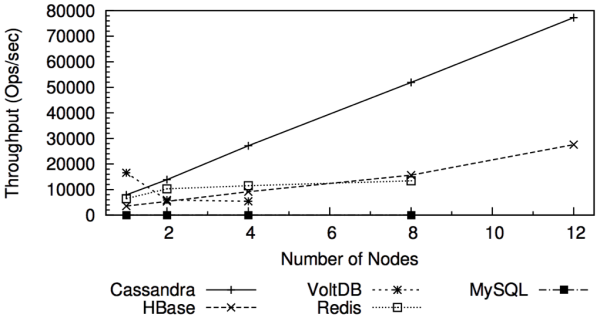
\includegraphics[scale=.5]{cassathpt.png}
	    \caption{Cassandra Performance\cite{cassathpt}.} 
	  \end{figure}
      
      \section{Cassandra C Client}
      \paragraph\
      Cassandra C client is a wrapper around Cassandra Python client that is Pycassa. I used C-Python API
      to write wrapper around Python's Pycassa API.   
%\chapter{\label{chap:Implementation}Results and Analysis}
%\paragraph\
In this chapter we have tested scalability of \emph{ntop} with RRDTool, \emph{ntop} with cassandra and  Open vSwitch with Cassandra. We have used 32KB, 64KB, 128KB socket buffer for \emph{ntop} and SWSR IPC buffer for Open vSwitch to test behavior of our solutions. Using \emph{netperf} \cite{netperf} tool we have generated traffic. 

\paragraph\
In the first section we present \emph{netperf} tool. In Section \ref{testbed}, we present our test environment. We have presented results and
discussion in the Section \ref{result_and_Dis}. Finally we conclude with Section \ref{Result_conclusion}.

\section{\emph{netperf}} \label{etperf}
\paragraph\
	\emph{netperf} is a benchmark tool that can be use to measure various aspect of networking performance. The primary focus are bulk  data transfer and request/response performance using either TCP or UDP and the Berkeley Sockets interface. Using \emph{netperf} we can perform following 
	tests \cite{netperf}
	\begin{enumerate}
	 \item TCP and UDP unidirectional transfer and request/response over IPv4 and IPv6 using the Sockets interface. 
	 \item TCP and UDP unidirectional transfer and request/response over IPv4 using the XTI interface. 
	 \item Link-level unidirectional transfer and request/response using the DLPI interface. 
	 \item Unix domain sockets.
	 \item SCTP unidirectional transfer and request/response over IPv4 and IPv6 using the sockets interface. 
	\end{enumerate}
\paragraph\
	TCP Connect/Request/Response measures the performance of establishing a connection, exchanging a single request/response transaction, and tearing-down that connection. TCP\_CRR creates two new flow for every request/response transaction. In a TCP\_CRR performance test, a \emph{netperf} 	creates lots of flow which can be monitored by Open vSwitch or any other NetFlow enabled router/switch. Using TCP\_CRR we simulate a heavy loaded network in our lab. In the next section we present our testbed that uses \emph{netperf} for generating NetFlow packets for our tests. 

\section{Test Environment Setup} \label{testbed}
	Our test environment contains multiple components as described in the Table \ref{table_testbed}. We have use KVM, Open vSwitch to create virtual network that generates NetFlow packets using Open vSwitch. Figure \ref{figure_testbed} illustrate our experimental testbed. Each of our system Sys-1, 2, 3, 4 are running OpenSuse-12.2(Linux 3.4 kernel). Sys-1 and 2 are using latest version of KVM. Sys-1 and 2 have 5 virtual machines each of them running 25 \emph{netperf} clients.% Ma'am I'm not able form the next sentense properly
	one VM each from both Sys-1 and Sys-2 forms five pairs of VM. Each pairs of VM have 25 \emph{netperf} clients each sending traffic to each other. With 25 \emph{netperf} running on both Sys-1 and Sys-2, we get approximately 1000 NetFlow packets/second. Figure \ref{peakNetperf} illustrates out claim. So all together the testbed runs 250 \emph{netperf} clients. In the next section we describe about our tests that we have done using this testbed.
	\begin{table}
	\centering
	 \begin{tabular}{|l|l|}
	  \hline
	  \textbf{Component Name} & \textbf{Details/Version} \\ \hline
	  CPU   & Intel(R) Core(TM) i5-2400 CPU @ 3.10GHz. \\ \hline
	  Operating System & OpenSuse 12.2 \\ \hline
	  Linux Kernel & 3.4 \\ \hline
	  KVM          & kvm-1.1.1-1.8.1 \\ \hline
	  Open vSwitch & openvswitch-1.9.0(LTS) \\ \hline
	  \emph{netperf} & netperf-2.6 \\ \hline
	  \emph{ntop}    & ntop-5.0.1 \\ \hline
	  Cassandra      & Apache-cassndra-1.2.5 \\ \hline	  
	 \end{tabular}
	  \label{table_testbed}
	  \caption{Components of Our Testbed}
	\end{table}

	\begin{figure}[htb]
	  \centering
	  \includegraphics[scale=.3]{testbed}
	  \caption{Evaluation Testbed } 
	  \label{figure_testbed}
	\end{figure}
	\begin{figure}[htb]
	  \centering
	  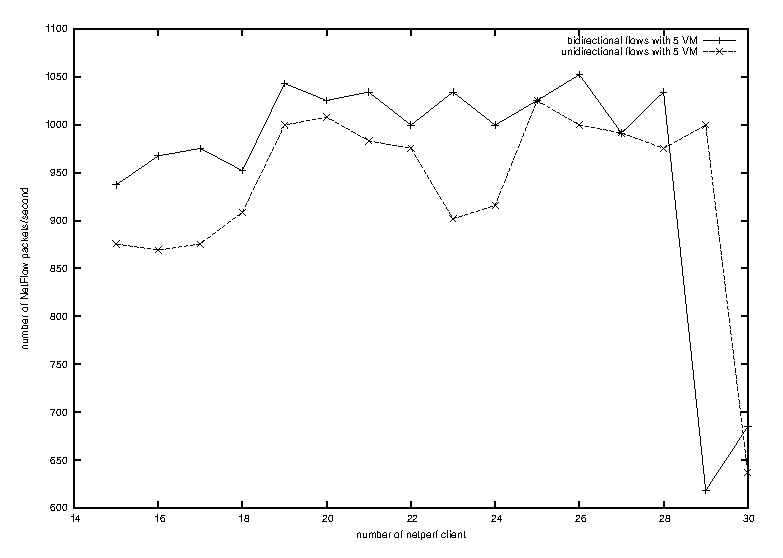
\includegraphics[scale=1]{data/peaknetperf}
	  \caption{NetFlow Packet generated with \emph{netperf}} 
	  \label{peakNetperf}
	\end{figure}
	
\section{Analysis and Discussion of Test Results} \label{result_and_Dis}
\paragraph\
	We have tested scalability of the following conditions with various socket buffer SWSR IPC buffer sizes. 
	\begin{enumerate}
	 \item \emph{ntop} and RRDTool.
	 \item \emph{ntop} storing NetFlow records to Cassandra.
	 \item Open vSwitch storing into NetFlow records directly into Cassandra.
	\end{enumerate}
	\paragraph{\emph{ntop} and RRDTool:} In this test, we have generated NetFlow packets with Sys-1 and Sys-2 and Open vSwitch 
	of Sys-2 exports NetFlow packets to \emph{ntop} running on Sys-3. \emph{ntop} uses RRDTool to analysis and store NetFlow
	statistics.
	\paragraph{\emph{ntop} and Cassandra:} In this test, we have run the similar test excepts Cassandra us used to store NetFlow records.
	\paragraph{Open vSwitch and Cassandra:} In this test, Open vSwitch stores NetFlow records directly using NfCassaStore as described in pervious chapter.
	 
	\subsection{Analysis of the Graphs}
	\paragraph\
		Figure \ref{graph32}, \ref{graph64} and \ref{graph128} illustrate about number of packet drops in all three test cases with buffer size 32KB, 64KB and 128KB. Number of drops with RRDTool is very less with respect to other two.
		Open vSwitch with Cassandra tests improves better than \emph{ntop} storing into Cassandra if we increase amount of buffer. 
	\begin{figure}[!htb]
	    \centering
	    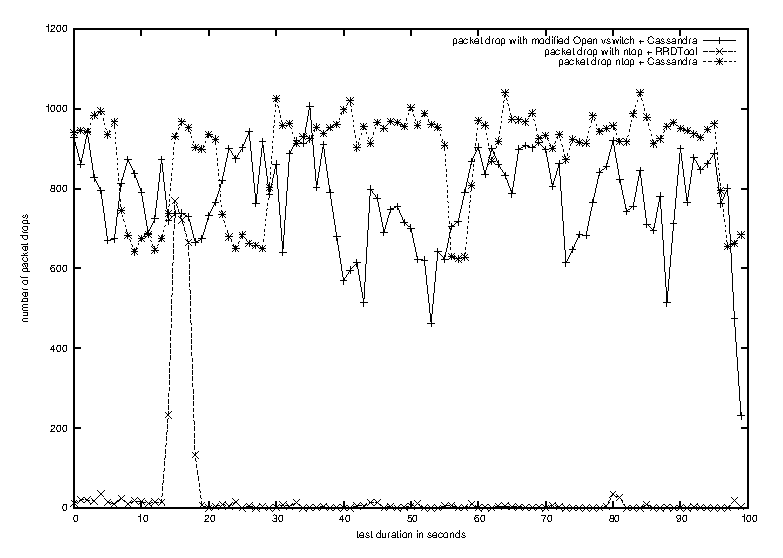
\includegraphics[scale=1]{data/out32}
	    \caption{Packet Drops with 32 KB Socket and IPC buffer size} 
	    \label{graph32}
	  \end{figure}
	
	  \begin{figure}[!htb]
	    \centering
	    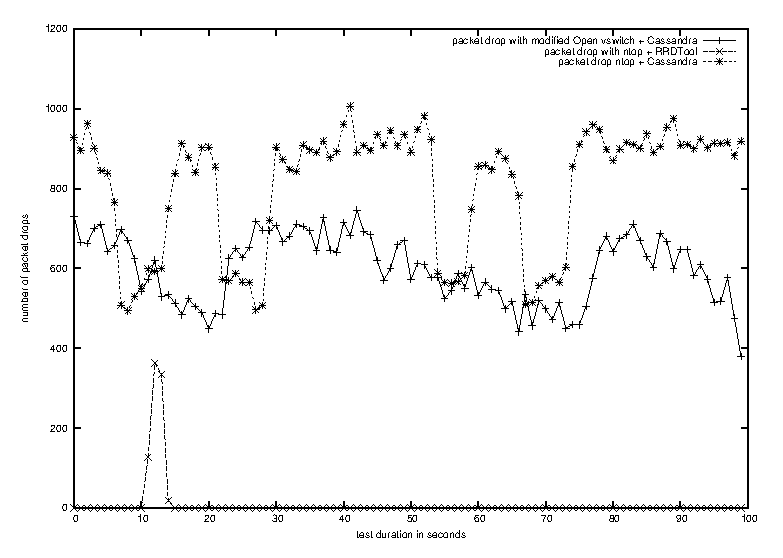
\includegraphics[scale=1]{data/out64}
	    \caption{Packet Drops with 64 KB Socket and IPC buffer size } 
	  \label{graph64}
	  \end{figure}
	  
	  \begin{figure}[!htb]
	    \centering
	    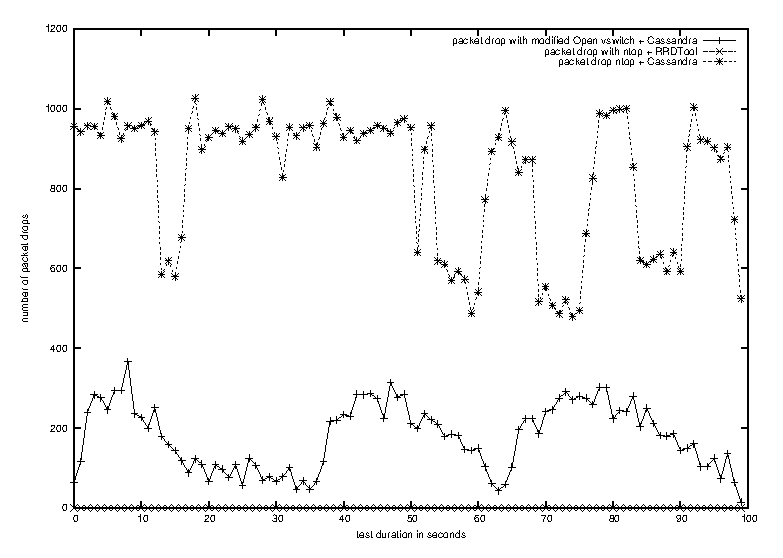
\includegraphics[scale=1]{data/out128}
	    \caption{Packet Drops with 128 KB Socket and IPC buffer size} 
	    \label{graph128}
	  \end{figure}
	  If we look at the detail operations that take place during our three tests, we may get more insights to analyze the results.
	  Operations done by \emph{ntop} with RRDTool:
	  \begin{enumerate}
	   \item Read NetFlow Packets from socket.
	   \item Analysis NetFlow packets 
	   \item Store NetFlow statistics into RRD with disk write.
	  \end{enumerate}
	  \emph{ntop} with Cassandra does similar operations except it stores NetFlow records into Cassandra using our Cassandra C client.
	  On the other hand Open vSwitch use \emph{Pycassa} to store NetFlow records into Cassandra. In both case, \emph{ntop} with RRDTool and Open vSwitch with Cassandra, a NetFlow packet pass thorugh network once and then stored into disk. In \emph{ntop} with Cassandra test, a Netflow packet has to pass through network twice, that explains why \emph{ntop} with Cassandra drops more packets than other two. \emph{ntop} with RRDTool is faster because RRDTool is written in c and dynamically linked with \emph{ntop}. Open vSwitch use Python, which is interpreted language and slower than
	  C.
	  \emph{ntop} with Cassandra does not improve its performance much with compare with Open vSwitch even we increase Socket buffer size.
	  \emph{ntop} uses our own Cassandra C client for storing data into Cassandra. Cassandra C client has pass through multiple layers of API calls (C-Python API, $Pycassa$ API, thrift API)	before reaching to Cassandra which is one reason for bad performance of \emph{ntop} with Cassandra. 
	  \paragraph\
	  
	  
	  

	  
\section{Conclusion} \label{Result_conclusion}
%\chapter{\label{chap:conclusion}Conclusions and Future Work}
%\section{Conclusions}
\paragraph\
Providing QoS in MANETs is a challenging task. Many solutions have been proposed but the solutions which are using resources efficiently are not scalable and the solutions which are scalable are not using resources efficiently. So we proposed a solution to achieve both the things. The proposed solution is a cross-layer QoS-aware routing protocol that supports multiple classes of service. It allocates resources to each class dynamically. It maintains per flow state information but provides per QoS level granularity. So fewer number of meters, policers and queues are required. In our scheme the source node acts as an edge router- metering, marking and conditioning of data packets. Other nodes act as core routers. We are implemented the scheme in \textit{ns-2.29} by extending Dynamic Source Routing(DSR) protocol. We compared our scheme with ASAP and SWAN in terms of call acceptance ratio, packet delivery ratio, throughput, latency to start data plane operations and average end-to-end delay.

\paragraph\
Simulation results show that our scheme has achieved throughput close to ASAP while using fewer meters, policers and queues. Results also show that call acceptance ratio of our scheme is higher than ASAP. From the results we can also observe that our scheme gives QoS guarantee to the flows when congestion occurs whereas SWAN does not. Latency to start data plane operations is also acceptable in our scheme. Average end-to-end delay for our scheme is less than that of both ASAP and SWAN. Overall, we are performing better than ASAP and SWAN. 
\pagebreak

\section{Future Work}
\paragraph\
We can do some optimizations and extensions to our scheme. Those are
\begin{itemize}
\item \textit{Local path repairing} : Actually in our scheme whenever route break occurs, again source only will find the new route. So if intermediate nodes find the new route instead of the source, we can reduce the packet loss.
\item Efficient measurement of available bandwidth by considering neighborhood information.
\item Our scheme only concentrated on bandwidth provisioning. We can also extend it to delay constraint. From the results we can observe that the average end-to-end delay for our scheme is less. So if we consider delay constraint during route discovery process, we may achieve that also as already our scheme has less end-to-end delay.
\end{itemize}

%\appendix
%\chapter{\label{chap:appendix} Design of the New Self-Organized Clustering Algorithm}
%\input{appendix.tex}
%\chapter{\label{chap:appendix} Modifications in \textit{ns-2} source code}
%\input{appendix_mod.tex}
\nocite{*}
\bibliographystyle{PhDbiblio-bold}
\newpage
\addcontentsline{toc}{chapter}{Bibliography}
\bibliography{ref.bib}
\newpage
\addcontentsline{toc}{chapter}{Index}
%\printindex
%\end{large}
\end{document}
